\documentclass{letter}
\usepackage[a4paper,left=2.5cm, right=2.5cm, top=2cm, bottom=2cm]{geometry}

% package imports
% ---------------

\usepackage[english]{babel} % for correct language and hyphenation and stuff
\usepackage{calc}           % for easier length calculations (infix notation)
\usepackage{enumitem}       % for configuring list environments
\usepackage{fancyhdr}       % for setting header and footer
\usepackage{fontspec}       % for fonts
\usepackage{geometry}       % for setting margins (\newgeometry)
\usepackage{graphicx}       % for pictures
\usepackage{microtype}      % for microtypography stuff
\usepackage{xcolor}         % for colours
\usepackage{outlines}
\usepackage{roboto}
\usepackage{lipsum}
\usepackage[hidelinks]{hyperref}
\usepackage{xspace}

% font families
\defaultfontfeatures{Ligatures=TeX} % reportedly a good idea, see https://tex.stackexchange.com/a/37251

% \newfontfamily{\cvnamefont}{Roboto Medium}
% \newfontfamily{\cvsectionfont}{Roboto Medium}
% \newfontfamily{\cvtitlefont}{Roboto Regular}
% \newfontfamily{\cvdurationfont}{Roboto Light Italic}
% \newfontfamily{\cvheadingfont}{Roboto Regular}
% \setmainfont{Roboto Light}

% \setmainfont{RobotoMonoNerdFont}[
%     Path=\string~/.local/share/fonts/NerdFonts/,
%     Extension = .ttf,
%     UprightFont=*-Regular,
%     BoldFont=*-Bold,
%     ItalicFont=*-Italic,
%     BoldItalicFont=*-BoldItalic
%     ]

\newcommand{\thesisname}{Parametric analysis of actuator discs for wind turbine simulation\xspace}
\newcommand{\phdtitle}{Doctoral student in computational fluid dynamics of multiphase flows\xspace}
\newcommand{\phddivision}{Department of Engineering Mechanics, KTH University\xspace}

\address{Buenos Aires \\ Argentina}
\signature{
  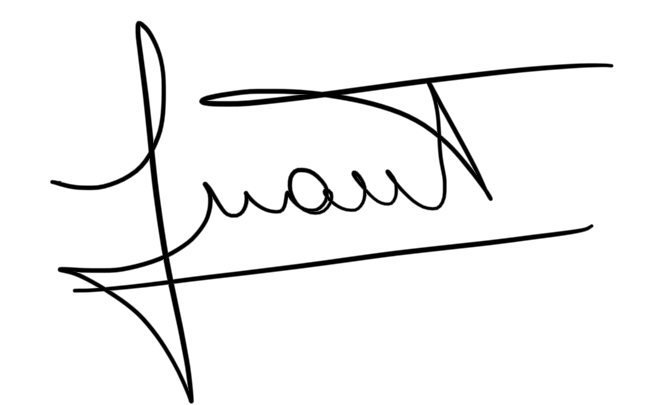
\includegraphics[width=4cm]{../../../../firma-JIT.png} \\
  Juan Ignacio Teich \\
  \href{mailto:juanignacioteich@gmail.com}{juanignacioteich@gmail.com} \\
  \href{mailto:jteich@fi.uba.ar}{jteich@fi.uba.ar} \\
  +54 9 11 6491 6389
  }
\begin{document}

\begin{letter}{}
\opening{Dear members of the selection committe,}

My name is Juan Ignacio Teich, and I am writing to express my strong interest in the \phdtitle at the \phddivision.  
  % With a background in CFD simulation in both academia and industry and having completed a 6 year Degree in Mechanical Engineering at the University of Buenos Aires (equivalent to a Master's degree in Europe), I am confident that my profile and experience align well with your PhD position.
  With a background in CFD simulation in both academia and industry and having completed a 6 year Degree in Mechanical Engineering at the University of Buenos Aires (equivalent to both a BSc and MSc in Europe), I am confident that my profile and experience align well with your PhD position.

At the moment, I am working at Nucleoelétrica Argentina S.A., the company that operates and designs nuclear plants in Argentina, as a Thermohydraulic Design Engineer. In this role my key responsibilities are to perform thermohydraulic analyses, mainly via CFD, to either validate key accident events or analyze unusual behaviors of components in the nuclear plant. Additionally, I have refactored and enhanced an in-house software to model water hammer phenomena using the Method of Characteristics, both for incompressible and compressible flows in complex pipe systems. 

Previously, I worked on my Engineering thesis titled '\thesisname', directed by Alejandro Otero and Dimas Barile, from the Renewable Energies Research Group at CSC (Center of Computational Simulations, CONICET) in Buenos Aires. 
    The main focus of the thesis was to compare the different models of actuator discs (a method to model wind turbines cost-efficiently) available. 
  The project involved a comprehensive literature review on the actuator disk models available, then coding them into OpenFOAM, simulating multiple validation cases on a cluster used in wind turbine modeling, and comparing the results to establish the advantages and disadvantages of each model.  

Through its development, I acquired and applied skills in OpenFOAM, as well as Python scripting for post-processing the output data from the CFD simulation.
    Additionally, in order to analyze actuator discs besides the ones developed within the research group, I learned C++ programming to understand and modify OpenFOAM’s source code, enabling me to develop my own actuator discs for comparison across multiple parameters.
The performance of the developed actuator disc models was evaluated in uniform inlet flow and atmospheric boundary layer conditions, considering wake interference in setups commonly observed in the literature. Finally, a brief comparison of computational costs was also included.

Additionally, during the first 6 months of my thesis, I worked at Stämm Biotech, an Argentine biotechnology startup, carrying out the role of 'Numeric Simulations Specialist'. 
  This role allowed me to further enhance my OpenFOAM skills, particularly with its meshing tool snappyHexMesh, extending their application in a different setting than wind power simulation. 
  Furthermore, I gained knowledge and practice in Object-Oriented Programming, both in further developing in-house simulation programs and applying them in my own post-processing scripts. 
  This role provided valuable interdisciplinary experiences, learning from people with backgrounds as varied as Biology, Chemistry, and Software Engineering, as well as teaching them from my own expertise in my field of study.
  % This position has been of importance for being able to apply CFD in an environment of industry rather than academia, which I think will be of great value in your PhD programme in conjunction with Vattenfall.

My Degree is in Mechanical Engineering, a 6 year Degree similar to both a BSc and MSc in Europe.
The curriculum covers a broad range of technical subjects regarding Mechanical Engineering, including but not limited to engineering materials, fluid dynamics, heat and mass transfer, structural design and turbomachinery. 
I chose to specialize in Computational Simulations, taking elective courses in Finite Element Analysis and its applications to solids and fluids.
This allowed me to have the solid foundation to then carry out my thesis in CFD and work in industry.
  
I have a strong interest in pursuing a PhD in Europe, as it represents an opportunity to carry out research and deepen my specialization in CFD and its development while staying connected to the practical needs of industry.
   I am eager to learn new programming skills that will enable me to further enhance and develop CFD methodologies, contributing to cutting-edge solutions in fluid dynamics.

The specific objectives of this PhD position greatly resonate with my academic and professional interests. 
    I would be thrilled to contribute to the field of CFD in the context of a PhD, combining my passion for research with my desire to advance CFD development. 
    The opportunity to apply data-driven tools to develop reduced-order models intrigues me, as it aligns with my passion for high-fidelity CFD simulations and their practical applications. 
    Additionally, I highly value KTH University as a great environment in which to pursue a PhD.
    % Additionally, the focus on applying machine learning to turbulence modeling excites me, being something I have been meaning to dive into as a way to accelerate CFD results. 


  % My interests are aligned with continuing learning, developing and applying my CFD simulation and development skills, both in academia and industry.
  % In particular, I have the desire to pursue a PhD to 
  % In particular, wind power simulation is a field of special interest and one in which I want to further advance in my career, which I have been lucky enough to get to work in through my Engineering thesis.

I have submitted my academic documents in Spanish, as they have not yet been legalized and translated into English. Due to the summer vacation period in Argentina, the administrative offices that handle this process have been closed since mid December to early February, which is why my documents are still pending. However, I find the position highly appealing and did not want to miss the opportunity to apply. I will submit the legalized and translated documents as soon as possible. 
  
  In case it is relevant for visa or other formal requirements, I posses EU citizenship, from Spain, as well as my Argentinian citizenship.

  Thank you for considering my application. I hope my profile is fit for the position and to hear from you in the near future.
\closing{Sincerely,}
\end{letter}

\end{document}
